\documentclass[amsmath,amssymb,twocolumn]{revtex4-1}

\usepackage{graphicx}% Include figure files
\usepackage{dcolumn}% Align table columns on decimal point
\usepackage{bm}% bold math
\usepackage[detect-all]{siunitx}
\usepackage{hyperref}% add hypertext capabilities
\usepackage{xr}
\externaldocument{si}
%\usepackage[mathlines]{lineno}% Enable numbering of text and display math
%\linenumbers\relax % Commence numbering lines

%\usepackage[showframe,%Uncomment any one of the following lines to test
%%scale=0.7, marginratio={1:1, 2:3}, ignoreall,% default settings
%%text={7in,10in},centering,
%%margin=1.5in,
%%total={6.5in,8.75in}, top=1.2in, left=0.9in, includefoot,
%%height=10in,a5paper,hmargin={3cm,0.8in},
%]{geometry}

\begin{document}

\preprint{APS/123-QED}

\title{Bayesian determination of the effect of a deep eutectic solvent on the
structure of lipid monolayers}% Force line breaks with \\%

\author{A.~R.~McCluskey}
\email{a.r.mccluskey@bath.ac.uk}
  \thanks{These authors have contributed equally to the work presented within}
  \altaffiliation[Also at ]{Diamond Light Source, Harwell Campus, Didcot,
  OX11 0DE, UK}
\affiliation{Department of Chemistry, University of Bath, Claverton Down,
Bath, BA2 7AY, UK}

\author{A.~Sanchez-Fernandez}
  \thanks{These authors have contributed equally to the work presented within}
  \altaffiliation[Also at ]{European Spallation Source, SE-211 00 Lund,
  Sweden}
  \altaffiliation[Present address ]{Department of Food Technology, Lund
  University, SE-211 00 Lund, Sweden}
\affiliation{Department of Chemistry, University of Bath, Claverton Down,
Bath, BA2 7AY, UK}

\author{K.~J.~Edler}
\affiliation{Department of Chemistry, University of Bath, Claverton Down,
Bath, BA2 7AY, UK}

\author{S.~C.~Parker}
\affiliation{Department of Chemistry, University of Bath, Claverton Down,
Bath, BA2 7AY, UK}

\author{A.~J.~Jackson}
  \altaffiliation[Also at ]{Department of Physical Chemistry,
  Lund University, SE-211 00 Lund, Sweden}
\affiliation{European Spallation Source, SE-211 00 Lund, Sweden}

\author{R.~A.~Campbell}
  \altaffiliation[Also at ]{Institut Laue-Langevin, 71 avenue des Martyrs,
  38000, Grenoble, France}
\affiliation{Division of Pharmacy and Optometry, University of Manchester,
Manchester, UK}

\author{T.~Arnold}
\email{tom.arnold@esss.se}
  \altaffiliation[Also at ]{ISIS Neutron and Muon Source, Science and
  Technology Facilities Council, Rutherford Appleton Laboratory, Harwell
  Oxford, Didcot OX11 OQX, UK; Diamond Light Source, Harwell Campus, Didcot,
  OX11 0DE, UK; Department of Chemistry, University of Bath, Claverton Down,
  Bath, BA2 7AY, UK}
\affiliation{European Spallation Source, SE-211 00 Lund, Sweden}


\date{\today}% It is always \today, today,
             %  but any date may be explicitly specified

\begin{abstract}
  In this work, we present the first example of the self-assembly of
  phospholipid monolayers at the interface between air and a non-aqueous
  liquid.
  Deep eutectic solvents are a novel class of environmentally friendly
  non-aqueous room temperature liquids with tunable properties, that have
  wide ranging potential applications and are capable of promoting the
  self-assembly of surfactant molecules.
  We use a chemically-consistent Bayesian modelling of X-ray and neutron
  reflectometry measurements to show that these monolayers broadly behave
  as they do on water.
  However, the ability of the deep eutectic solvent to interact with the
  phosphatidylglycerol lipid head, leads to an apparent increase in its
  volume compared to that observed in water.
  No such change was observed for the phosphocholine head, indicating that
  such interactions are head, and therefore solvent, specific.
  This has important implications for the potential uses of these solvents
  and for our understanding of how biomolecules behave in the absence of water.
\begin{description}
\item[Usage]
Electronic Supplementary Information (ESI) available: All analysis/plotting
scripts and figure files, allowing for a fully reproducible, and automated,
analysis workflow for the work presented is available at
\url{https://github.com/arm61/lipids_at_airdes} (DOI: 10.5281/zenodo.1464836)
under a CC-BY 4.0 license.
Reduced experimental datasets are available at
\url{https://researchdata.bath.ac.uk/id/eprint/548}, under a CC-BY 4.0 license.
\end{description}
\end{abstract}

%\keywords{Suggested keywords}%Use showkeys class option if keyword
                              %display desired
\maketitle

%\tableofcontents

Deep eutectic solvents (DES) are green, sustainable liquids that are obtained
through the combination of ionic species with compounds that act as hydrogen
bond donors, such as sugars, alcohols, amines, and carboxylic
acids\cite{Smith2014,Dai2013}.
The resulting extensive hydrogen bonding network is able to stabilise the
ionic species and allows the eutectic mixture to remain liquid at room
temperature\cite{Hammond2016,Hammond2017,Araujo2017}.
Through different combinations of the precursor materials, it is possible to
tune the solvent's physicochemical properties, such as
polarity\cite{Pandey2014}, viscosity and surface tension\cite{Smith2014},
network charge\cite{Zahn2016}, and
hydrophobicity\cite{Ribeiro2015,vanOsch2015}.
Recently DES have also been shown to exhibit a ``solvophobic'' effect through
the promotion of surfactant micelle
formation\cite{Sanchez-Fernandez2016,Arnold2015,Hsieh2018,Banjare2018},
phospholipid bilayer formation\cite{Bryant2017,Bryant2016,Gutierrez2009}, and
the ability to stabilise non-ionic polymer\cite{Sapir2016} and protein
conformations\cite{Sanchez-Fernandez2017}.

Phospholipid monolayers at the air/water interface have been widely studied
as simplistic models for biological membranes.
As such, they have been used to gain insight into many biological processes
that are technologically and medically relevant.
For example, investigations at the air/salt-water interface have identified
the importance that interactions between charged phospholipid heads and ions
present in solution have on the structure, monomer packing and stability of
the monolayer\cite{Mohwald1990,Kewalramani2010}.
However, the native environment for lipids in-vivo is far from a simple
aqueous solution.
In fact, it has been suggested\cite{Dai2013,Hammond2017} that DES might form
within the crowded cellular environment and could assist in solubilizing
biological species in an intermediate environment between that of the
hydrophobic phospholipid tails and highly polar water rich regions, thereby
assisting survival under extreme conditions such as freezing temperatures or
drought where the water content of cells is restricted.

This work presents the first observation of phospholipid monolayers at an
air-DES interface (or for that matter, any non-aqueous media, to the best of
the authors' knowledge).
We have used a chemically-consistent approach to model X-ray (XRR) and
neutron (NR) reflectometry measurements and thereby evaluate the effect of
this non-aqueous solvent on the structure of phospholipid monolayers.

Recent developments in computational resources and software have enabled
powerful methodologies and algorithms to be harnessed by those from
non-expert backgrounds.
This has benefitted significantly from open-source software projects such as
the Python language\cite{vanRossum1995} and the Jupyter notebooks
framework\cite{Kluyver2016}.
In the area of NR and XRR, the landscape of data-analysis software is diverse,
with a range of software packages available from a variety of sources;
refnx\cite{Nelson2018}, MOTOFIT\cite{Nelson2006}, Rascal\cite{HughesRascal}
Aurore\cite{Gerelli2016}, Refl1D\cite{Kienzle2011}, and GenX\cite{Bjorck2007}.

The use of a Python library, such as refnx, enables the implementation custom
models that contain chemically-relevant information as well as the
application of probability distribution function (PDF) sampling techniques.
The Python library emcee\cite{Foreman-Mackey2013} offers refnx to access the
Goodman \& Weare Affine Invariant Markov chain Monte Carlo (MCMC) Ensemble
method\cite{Goodman2010}.
This allows the sampling of the high-dimensionality parameter space, relevant
in reflectomety analysis, in a Bayesian fashion, where the new samples are
generated with consideration of those sampled previously\cite{Sivia2006}.
Bayesian inference gives an understanding of the PDF for the fitted
parameters and therefore estimations of their inverse uncertainties and
inter-parameter correlations.

%
\begin{figure}[b]
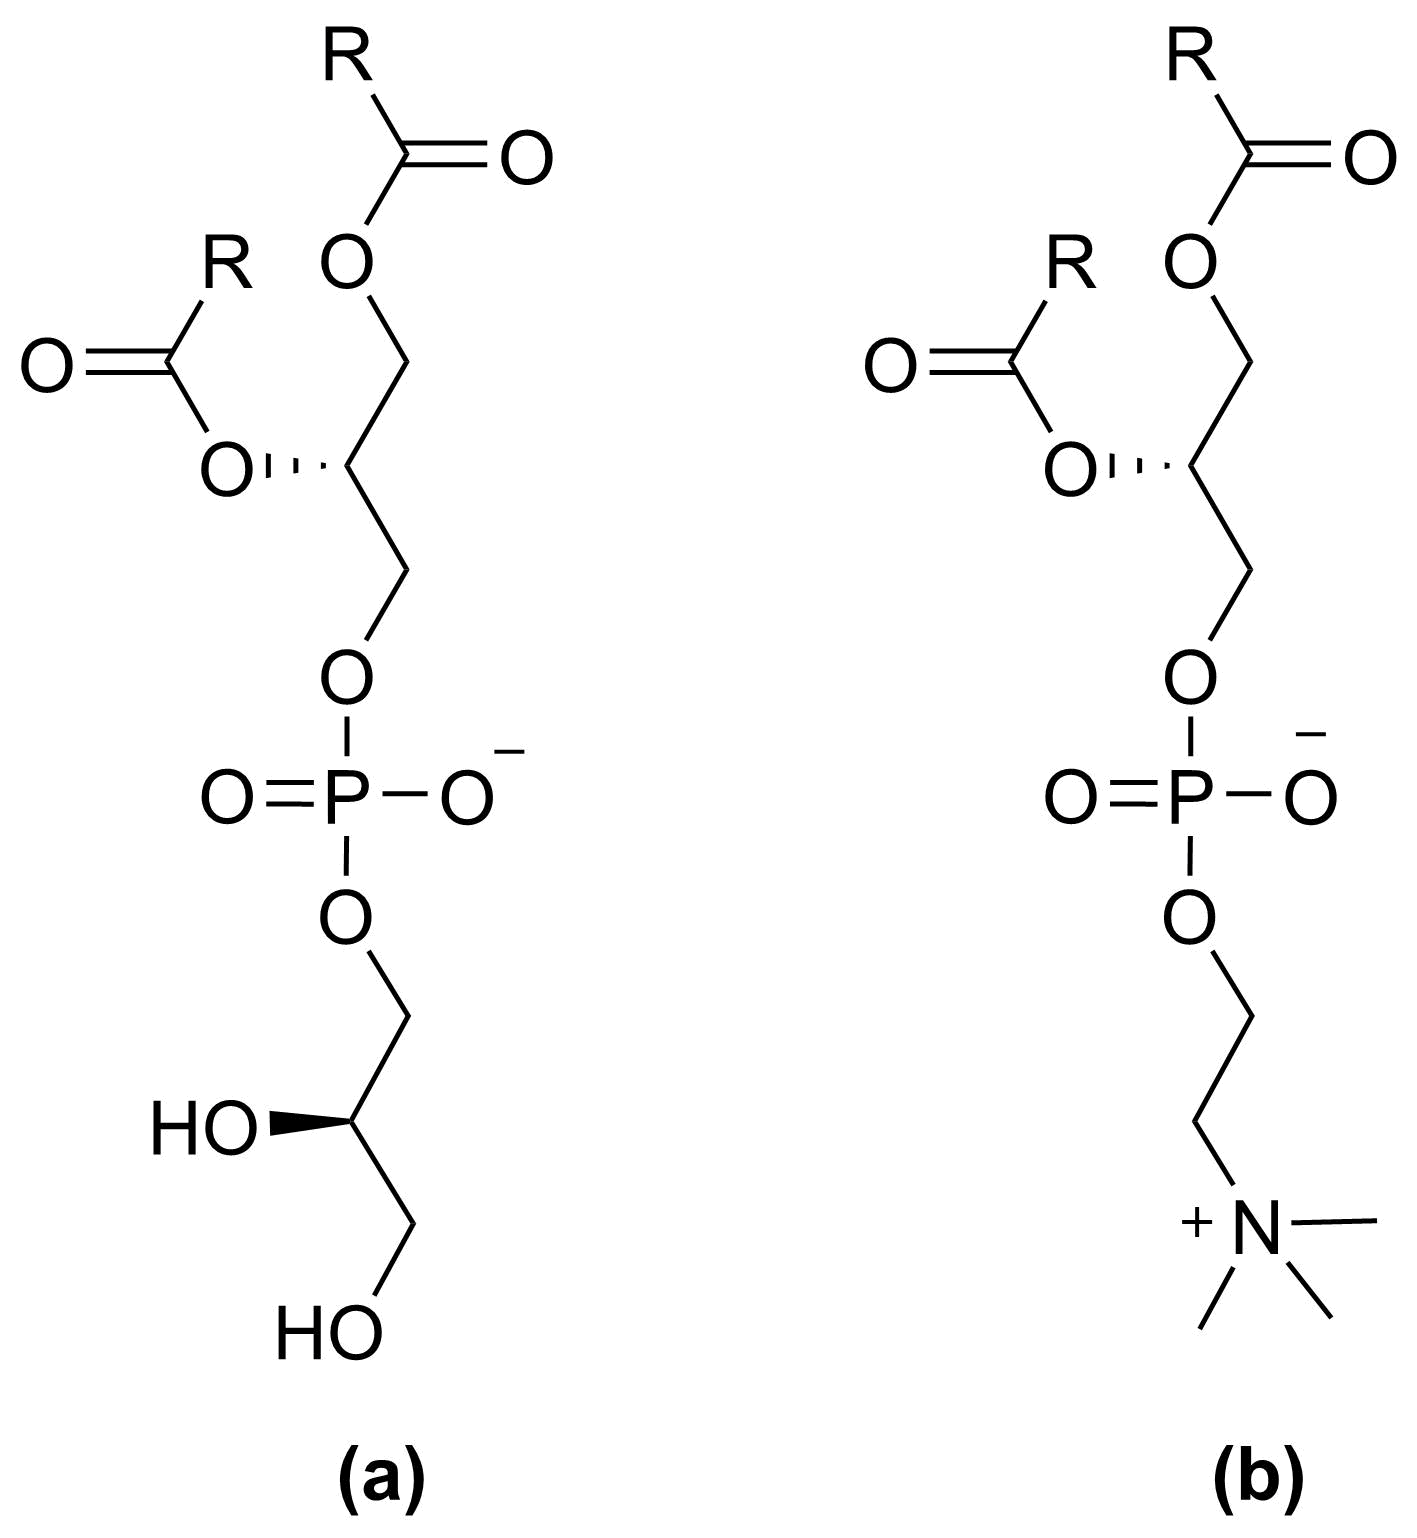
\includegraphics[width=0.3\textwidth]{figures/head_groups}
\caption{\label{fig:heads}\small The two lipid classes with different head
groups compared in this study, where R indicates the hydrocarbon tail;
(a) phosphatidylglycerol (PG), (b) phosphocholine (PC).}
\end{figure}
%
We report on measurements of four phospholipids monolayers, namely
1,2-dipalmitoyl-sn-glycero-3-phosphocholine (DPPC, C$_{16}$ tails),
1,2-dimyristoyl-sn-glycero-3-phosphocholine (DMPC, C$_{14}$ tails),
1,2-dilauroyl-sn-glycero-3-phosphocholine (DLPC, C$_{12}$ tails) and
1,2-dimyristoyl-sn-glycero-3-phospho-(1'-rac-glycerol)
(DMPG, C$_{14}$ tails), at the air-DES (1:2 choline choride:glycerol)
interface.
In contrast to many previous studies\cite{Mohwald1990,Kewalramani2010,
Bayerl1990,Johnson1991,Clifton2012,Helm1987,Daillant1990}, we have developed
a chemically-consistent model (detail in the ESI) that allows for the
co-refinement of reflectometry measurements at different surface pressure
and makes no assumption of the volume of the lipid head, $V_h$, or tail, $V_t$.
Instead these parameters were allowed to vary for each lipid while being
constrained to be self-consistent over different surface pressures in the
same phase; Liquid-Condensed (LC) for DPPC and Liquid-Expanded (LE) for
DMPC, DMPG and DLPC.
This model was required because we cannot assume that the electrostatic
interactions between lipid head and the solvent are the same in the DES and
in water. This may therefore influence the effective head volume which means
we cannot rely on the literature values (see ESI) derived from measurements
on or in water.
Furthermore, it is known that, on water, increased surface pressure and
associated LE-LC phase transitions lead to a compression of the lipid tail
volume\cite{Marsh2010,Small1984} and this compaction has not necessarily
been accounted for in the literature\cite{Campbell2018}.
Our approach avoids this issue by making no assumption about the molecular
volumes and only considering surface pressures that we believe to be in the
same phase.

%
\begin{figure}
	\centering
  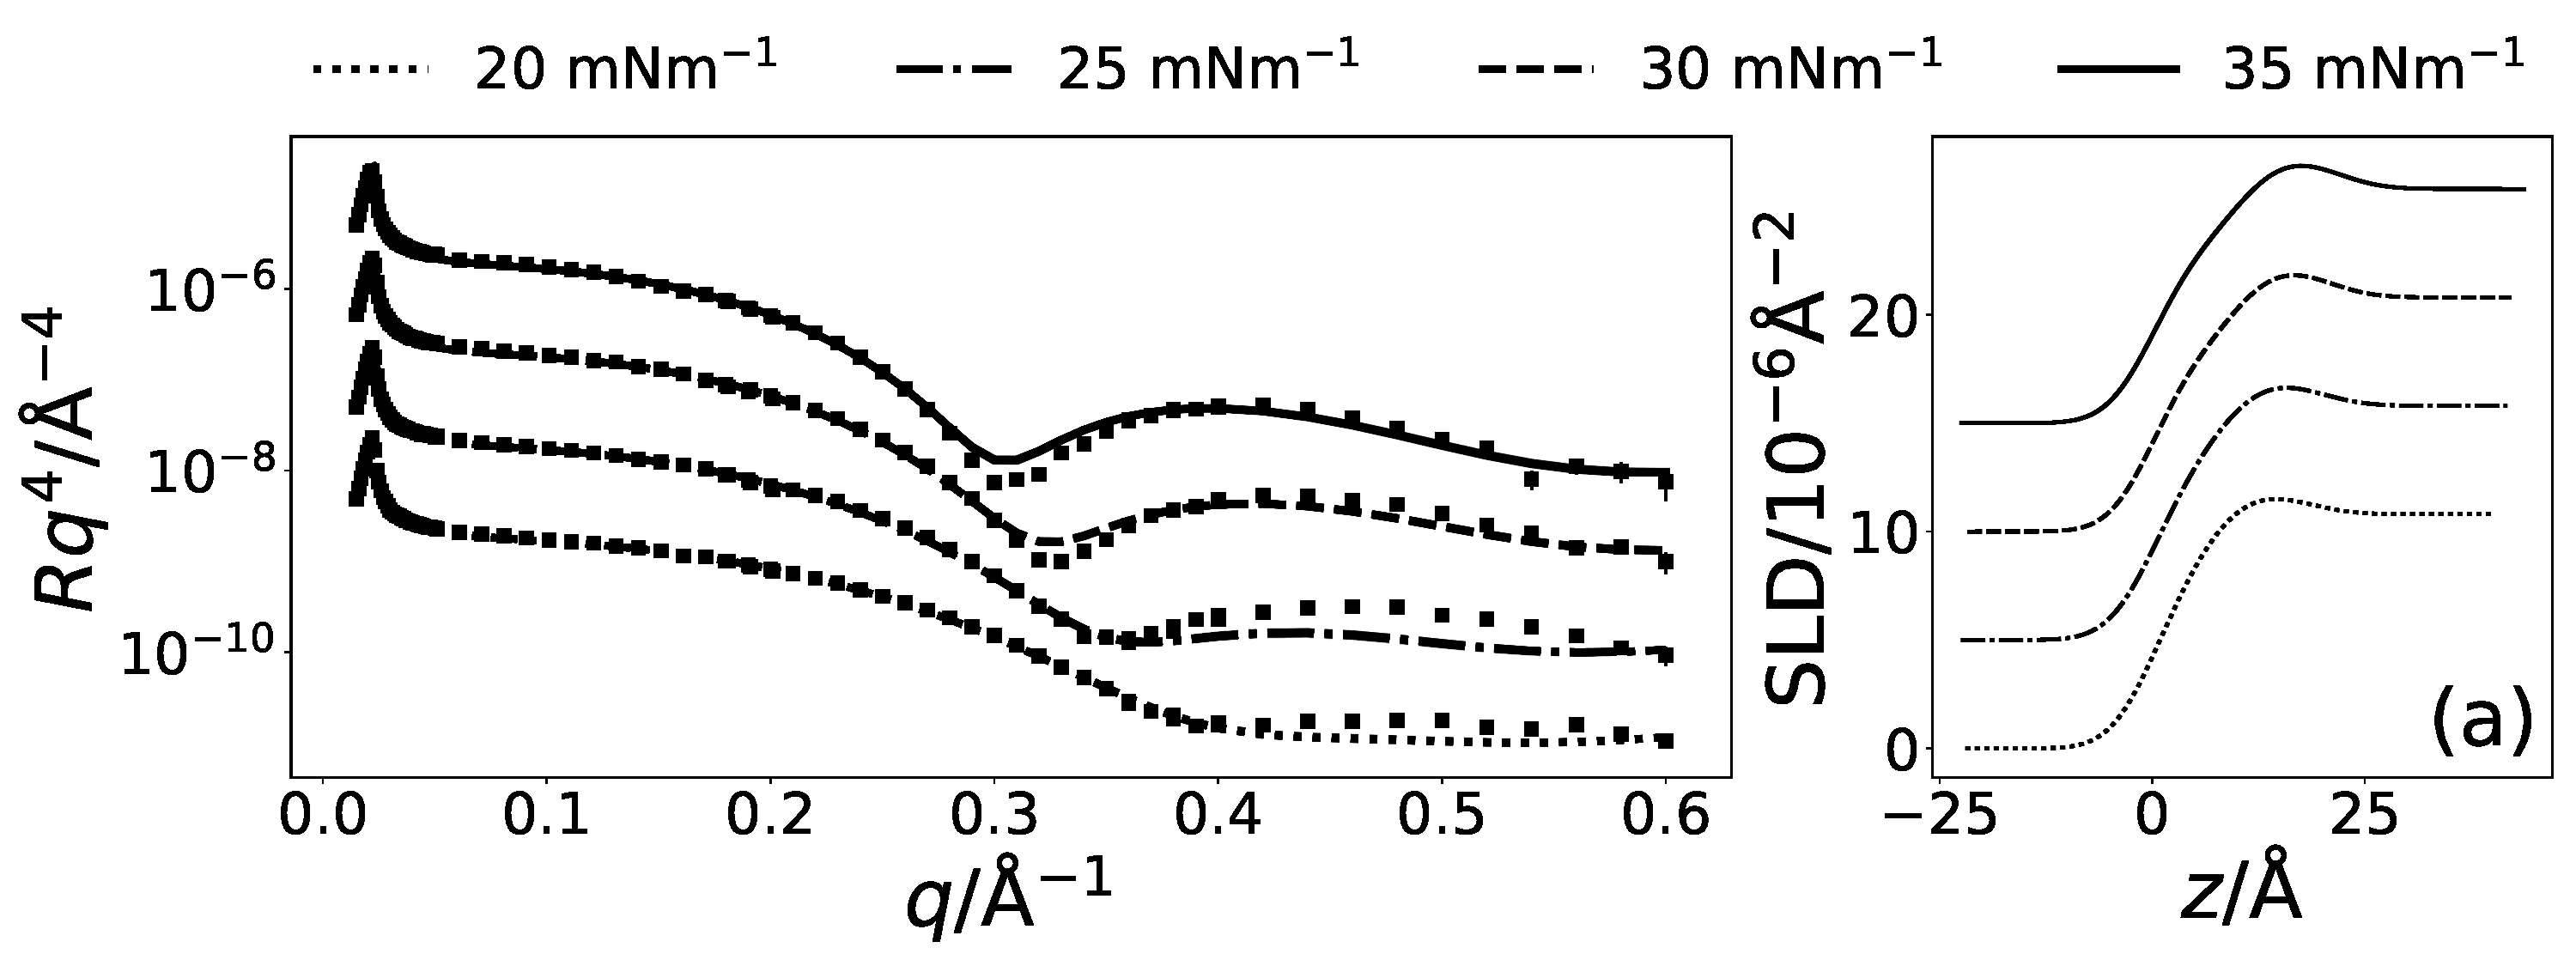
\includegraphics[width=0.45\textwidth]{figures/dlpc_ref_sld}
	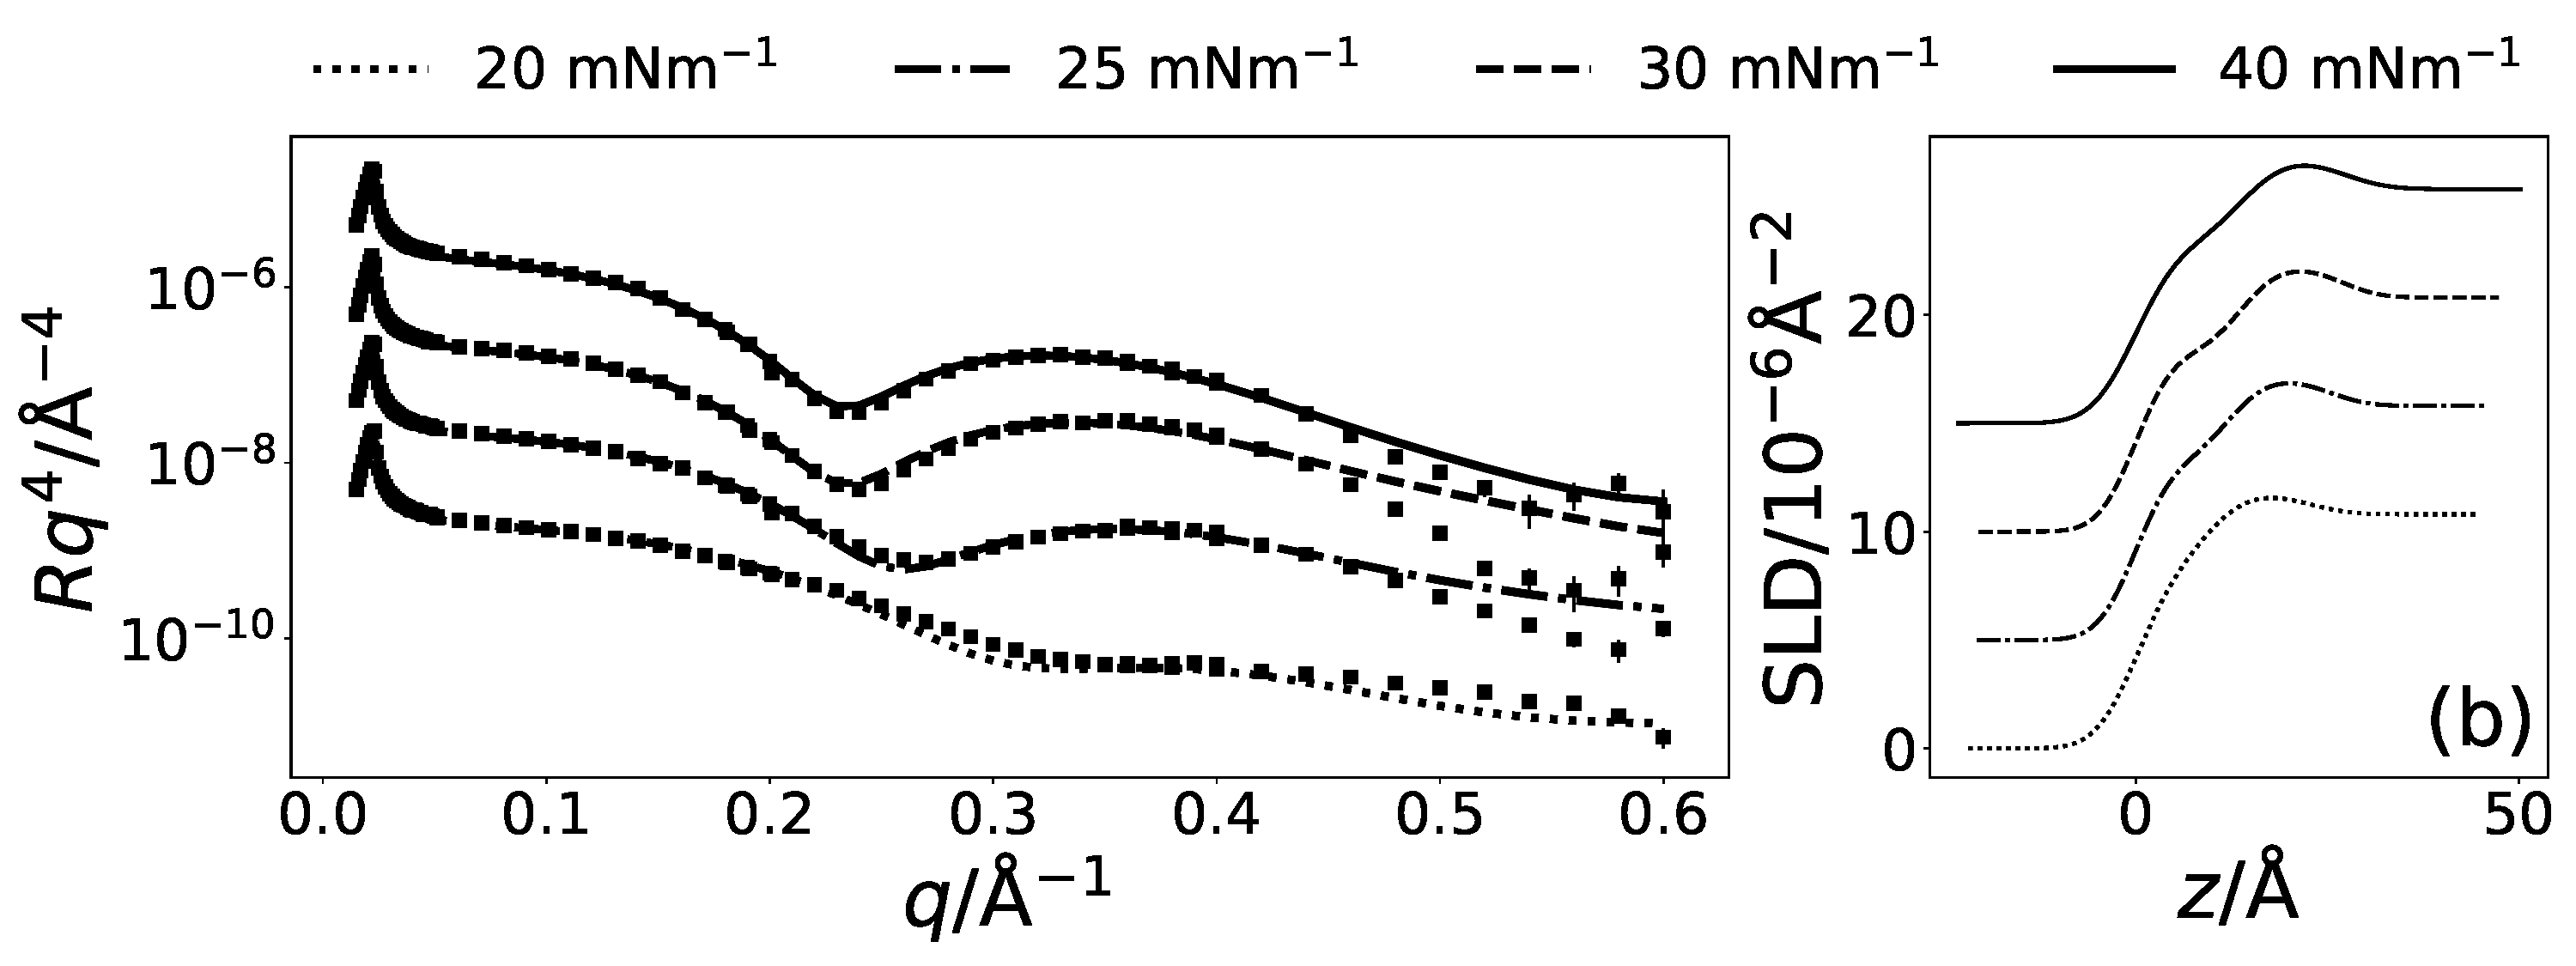
\includegraphics[width=0.45\textwidth]{figures/dmpc_ref_sld}
	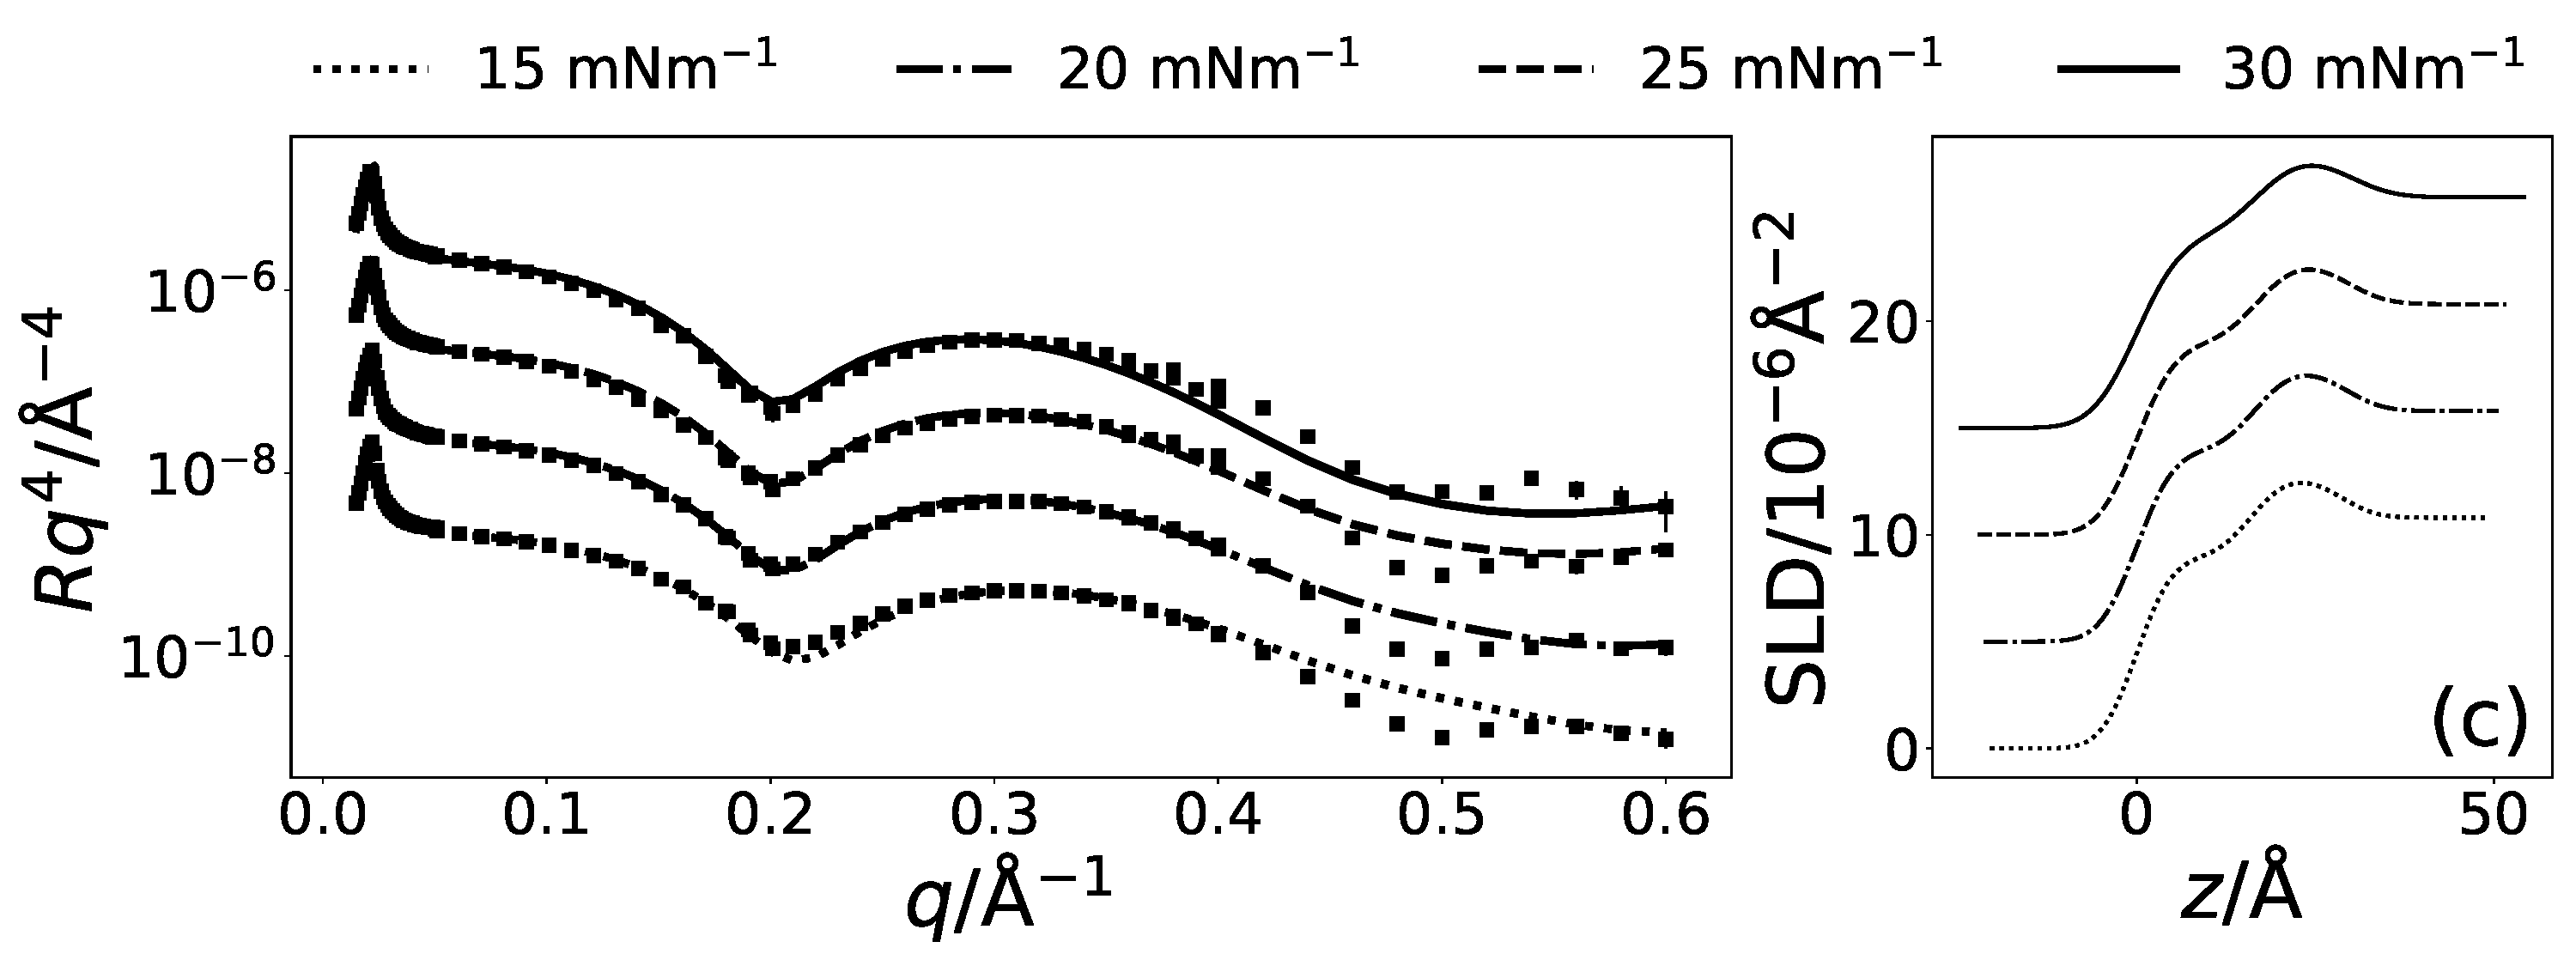
\includegraphics[width=0.45\textwidth]{figures/dppc_ref_sld}
	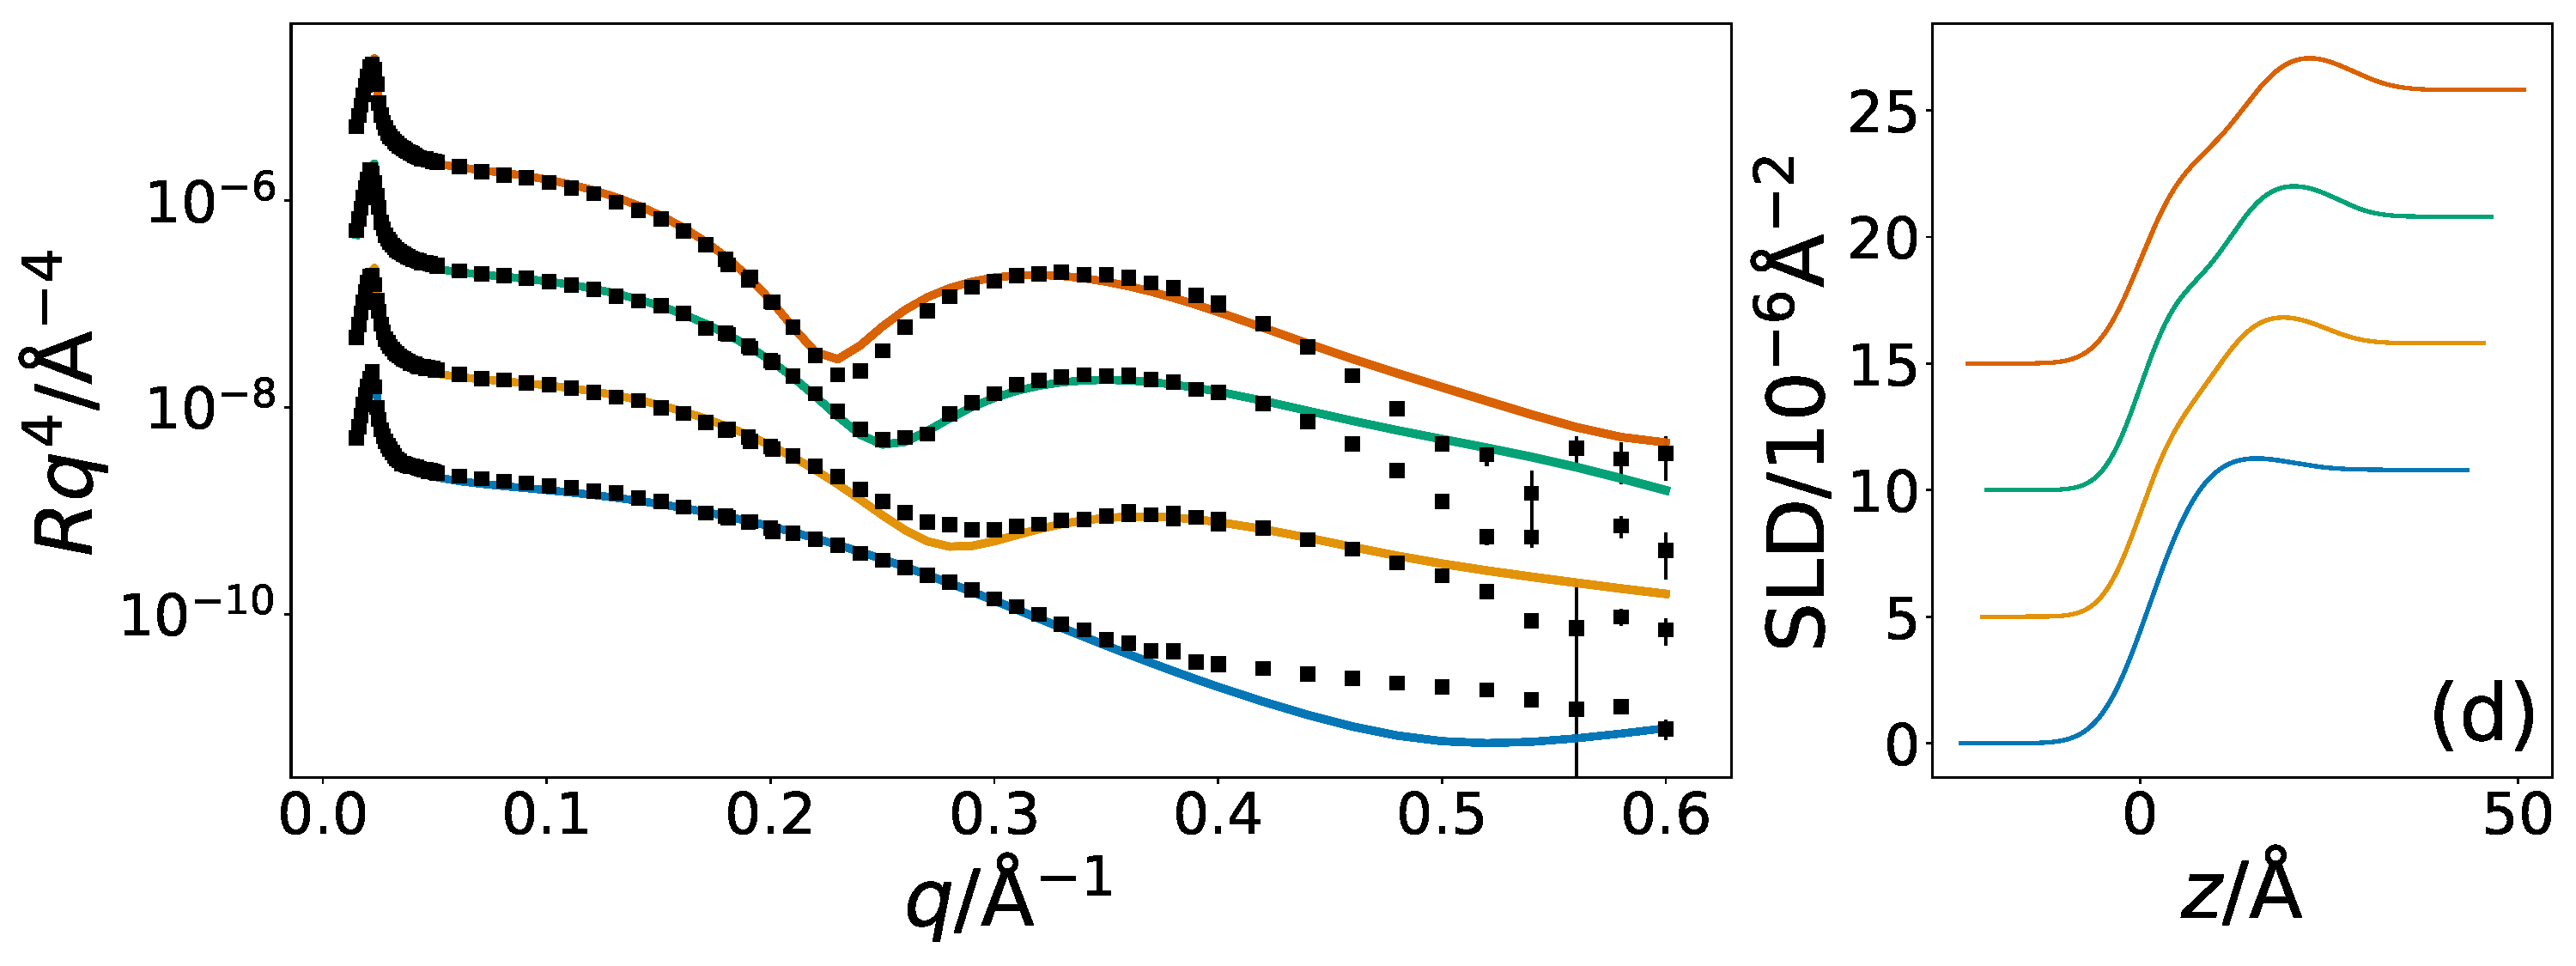
\includegraphics[width=0.45\textwidth]{figures/dmpg_ref_sld}
	\caption{\small The XRR profiles (left) and SLD profiles (right) for each
  of the four lipids; (a) DLPC, (b) DMPC, (c) DPPC, (d) DMPG, at the four
  measured surface pressures; see legend above each plot. The different
  surface pressure XRR profiles have been offset in the $y$-axis by an order
  of magnitude and SLD profiles offset in the $y$-axis by
  \SI{5e-6}{\per\square\angstrom}, for clarity.}
	\label{fig:lipids}
\end{figure}
%
Our model has more variables than we can uniquely fit with limited data.
In reflectometry the usual approach to this problem is to collect more
equivalent dataset with varying deuteration (NR). For reasons of cost and
practicality this was not possible in this work.
The other approach is to constrain the model so that the number of fitted
variables are reduced, and is the approach taken here.
To do this we add the constraint that a single tail volume can be used for
all surface pressures. To justify this we need to be sure that the lipids
remain in the same phase. On water this is can be demonstrated with a
Langmuir isotherm.
However, while we have confidence that the individual surface pressures
measured were reliable, we were unable to collect consistent Langmuir
isotherm measurements, due to the high viscosity of the DES.
This inconsistency means that we cannot be confident in the phase of the
lipids based on the surface pressure alone.
Instead we have used grazing incidence X-ray diffraction to confirm the
phases of DMPC and DPPC at \SI{30}{\milli\newton\per\meter}.
DPPC was found to be in the LC phase and DMPC in the LE phase at room
temperature for the surface pressures measured (see Section \ref{sec:gixd}).
We assume that DMPG and DLPC are also in the LE phase since there is no
reason to believe that the phase behaviour in these systems differs
significantly from DMPC at the same temperature.

The model, based on the standard two-layer model widely used for lipids on
water, was first fitted to the experimental XRR data.
The associated SLD profiles are shown in Figure \ref{fig:lipids} while
Table \ref{tab:liptab} presents the results of the PDF for each of the
varying parameters; the tail tilt angle, $\theta_t$, the interfacial
roughness, $\sigma$, the head and tail volumes, $V_h$ and $V_t$ respectively,
and the head layer thickness, $d_h$.
In order to constrain the fitting process only $\theta_t$ and $\sigma$ were
allowed to vary independently of surface pressure. The other parameters,
$V_h$, $V_t$ and $d_h$ were fitted to a single value for all of the surface
pressures measured for each lipid.

%
\begin{table}
	\caption{\label{tab:liptab} The best-fit values, and associated 95 \%
  confidence intervals for the varying parameters in the XRR models, at the
  \SI{30}{\milli\newton\per\meter}. The values of $d_t$ were found from the
  appropriate values of $\theta_t$ using Eqn. \ref{equ:tl} and the values for
  $\phi_h$ were obtained from the appropriate use of Eqn. \ref{equ:phih}.}
  \begin{ruledtabular}
	\begin{tabular}{ccccc}
    Lipid & DLPC & DMPC & DPPC & DMPG \\
    \hline
    $\theta_t$/\si{\degree} & \input{../output/dlpc/angle30.txt} &
    \input{../output/dmpc/angle30.txt} & \input{../output/dppc/angle30.txt} &
    \input{../output/dmpg/angle30.txt} \\
    $\sigma$/\si{\angstrom} & \input{../output/dlpc/rough30.txt} &
    \input{../output/dmpc/rough30.txt} & \input{../output/dppc/rough30.txt} &
    \input{../output/dmpg/rough30.txt} \\
    \hline
    $V_t$/\si{\cubic\angstrom} & \input{../output/dlpc/vt.txt} &
    \input{../output/dmpc/vt.txt} & \input{../output/dppc/vt.txt} &
    \input{../output/dmpg/vt.txt} \\
    $V_h$/\si{\cubic\angstrom} & \input{../output/dlpc/vh.txt} &
    \input{../output/dmpc/vh.txt} & \input{../output/dppc/vh.txt} &
    \input{../output/dmpg/vh.txt} \\
    $d_h$/\si{\angstrom} & \input{../output/dlpc/head.txt} &
    \input{../output/dmpc/head.txt} & \input{../output/dppc/head.txt} &
    \input{../output/dmpg/head.txt} \\
    \hline
    $\phi_h$/$\times10^{-2}$ & \input{../output/dlpc/solh30.txt} &
    \input{../output/dmpc/solh30.txt} & \input{../output/dppc/solh30.txt} &
    \input{../output/dmpg/solh30.txt} \\
    $d_t$/\si{\angstrom} & \input{../output/dlpc/tail30.txt} &
    \input{../output/dmpc/tail30.txt} & \input{../output/dppc/tail30.txt} &
    \input{../output/dmpg/tail30.txt} \\
	\end{tabular}
  \end{ruledtabular}
\end{table}
%

For each lipid, the tail layer thickness, $d_t$, increases with chain length
and in general agrees with the literature for monolayers on
water\cite{Mohwald1990,Vaknin1991}:
For DMPC, \input{../output/dmpc/tail30.txt}\si{\angstrom} at
\SI{30}{\milli\newton\per\meter} in DES compared with
$d_t=\SI{15.8}{\angstrom}$ at
\SI{30}{\milli\newton\per\meter}\cite{Johnson1991} in water, and for
DPPC \input{../output/dppc/tail30.txt}\si{\angstrom} at
\SI{30}{\milli\newton\per\meter} in DES compared with
$d_t=\SI{16.7}{\angstrom}$ at
\SI{40}{\milli\newton\per\meter}\cite{Helm1987} in water.
In all cases the surface roughness was found to be relatively high compared
to water.
This is expected because the absolute surface tension of the DES is less
than water, while a previous XRR measurement of pure choline
chloride:glycerol suggests a roughness of
3.3\si{\angstrom}\cite{Sanchez-Fernandez2016}, significantly higher than
the capillary wave roughness of water of about 2.8\si{\angstrom}.

Figure \ref{fig:lipresults} shows the tail layer thickness variation with
surface pressure. For DPPC and DMPC a plateau in thickness is reached at
\SI{25}{\milli\newton\per\meter} and \SI{30}{\milli\newton\per\meter}
respectively. Presumably a similar plateau would be seen for DMPG and DLPC
at higher pressures.
This phenomenon has been noted before for DMPC\cite{Bayerl1990} and
DPPC\cite{Campbell2018} at the air-water interface.
%
\begin{figure}
	\centering
  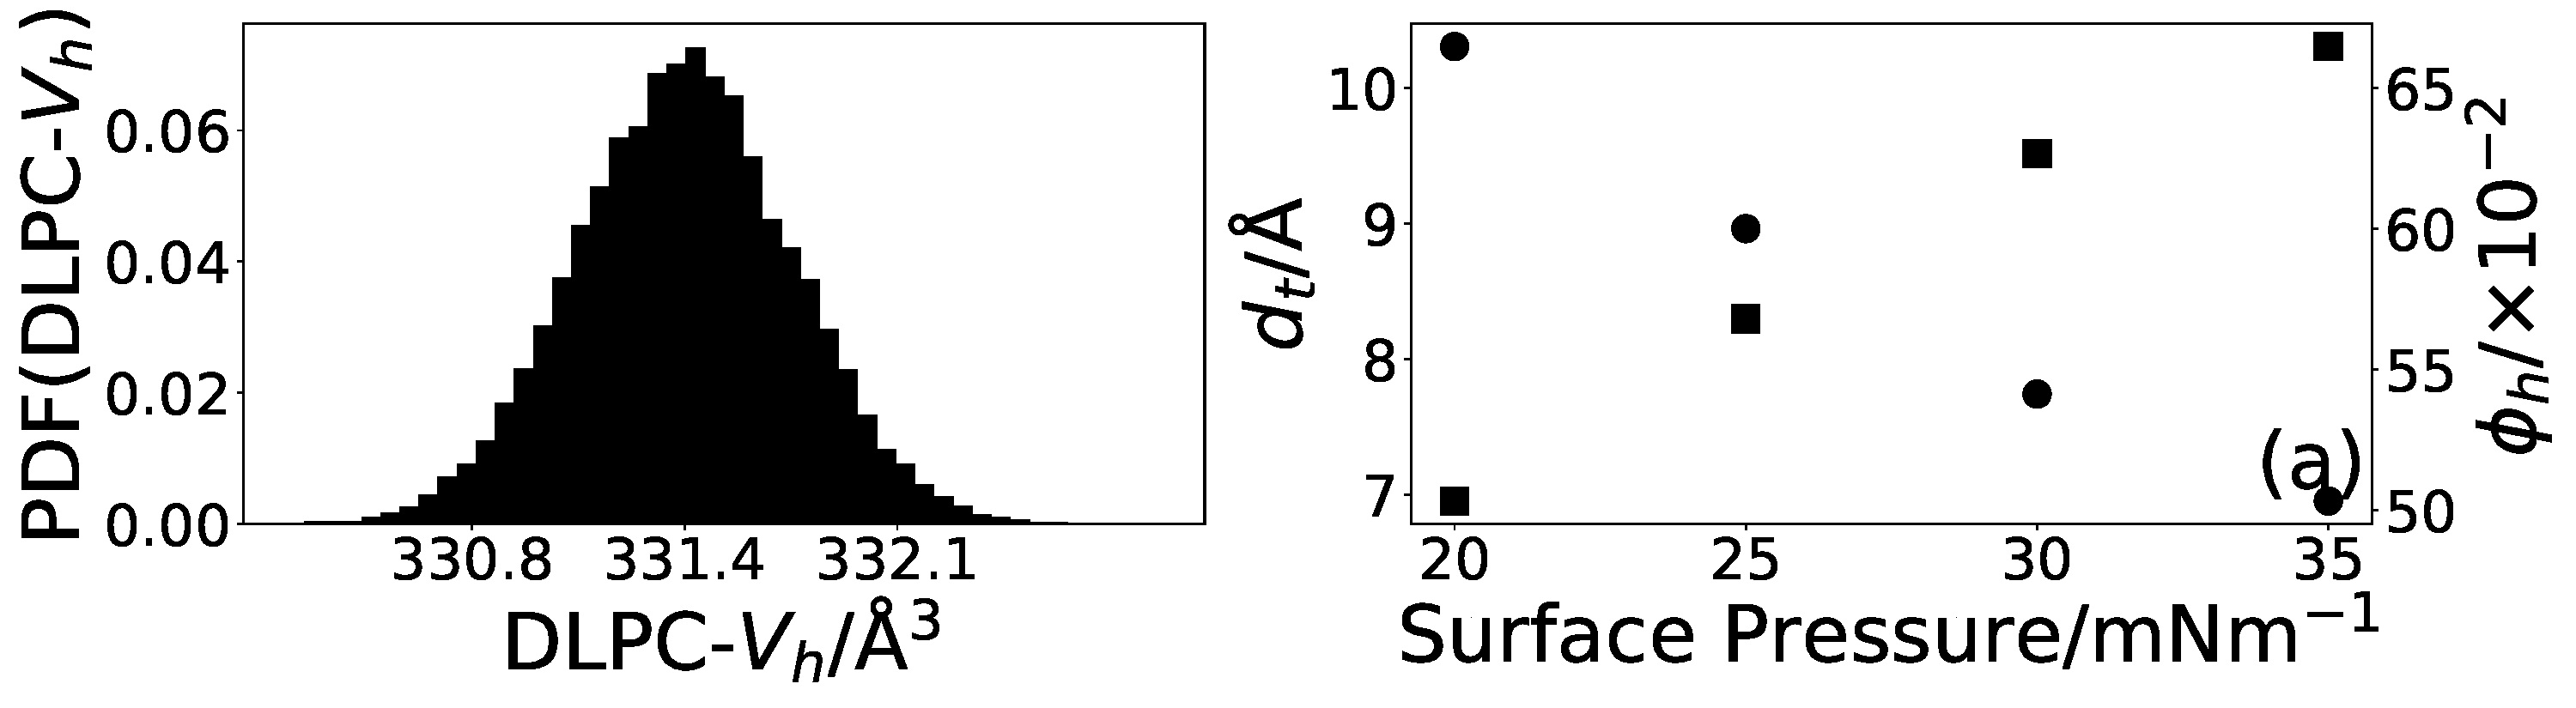
\includegraphics[width=0.45\textwidth]{figures/dlpc_vh_dt_phi}
	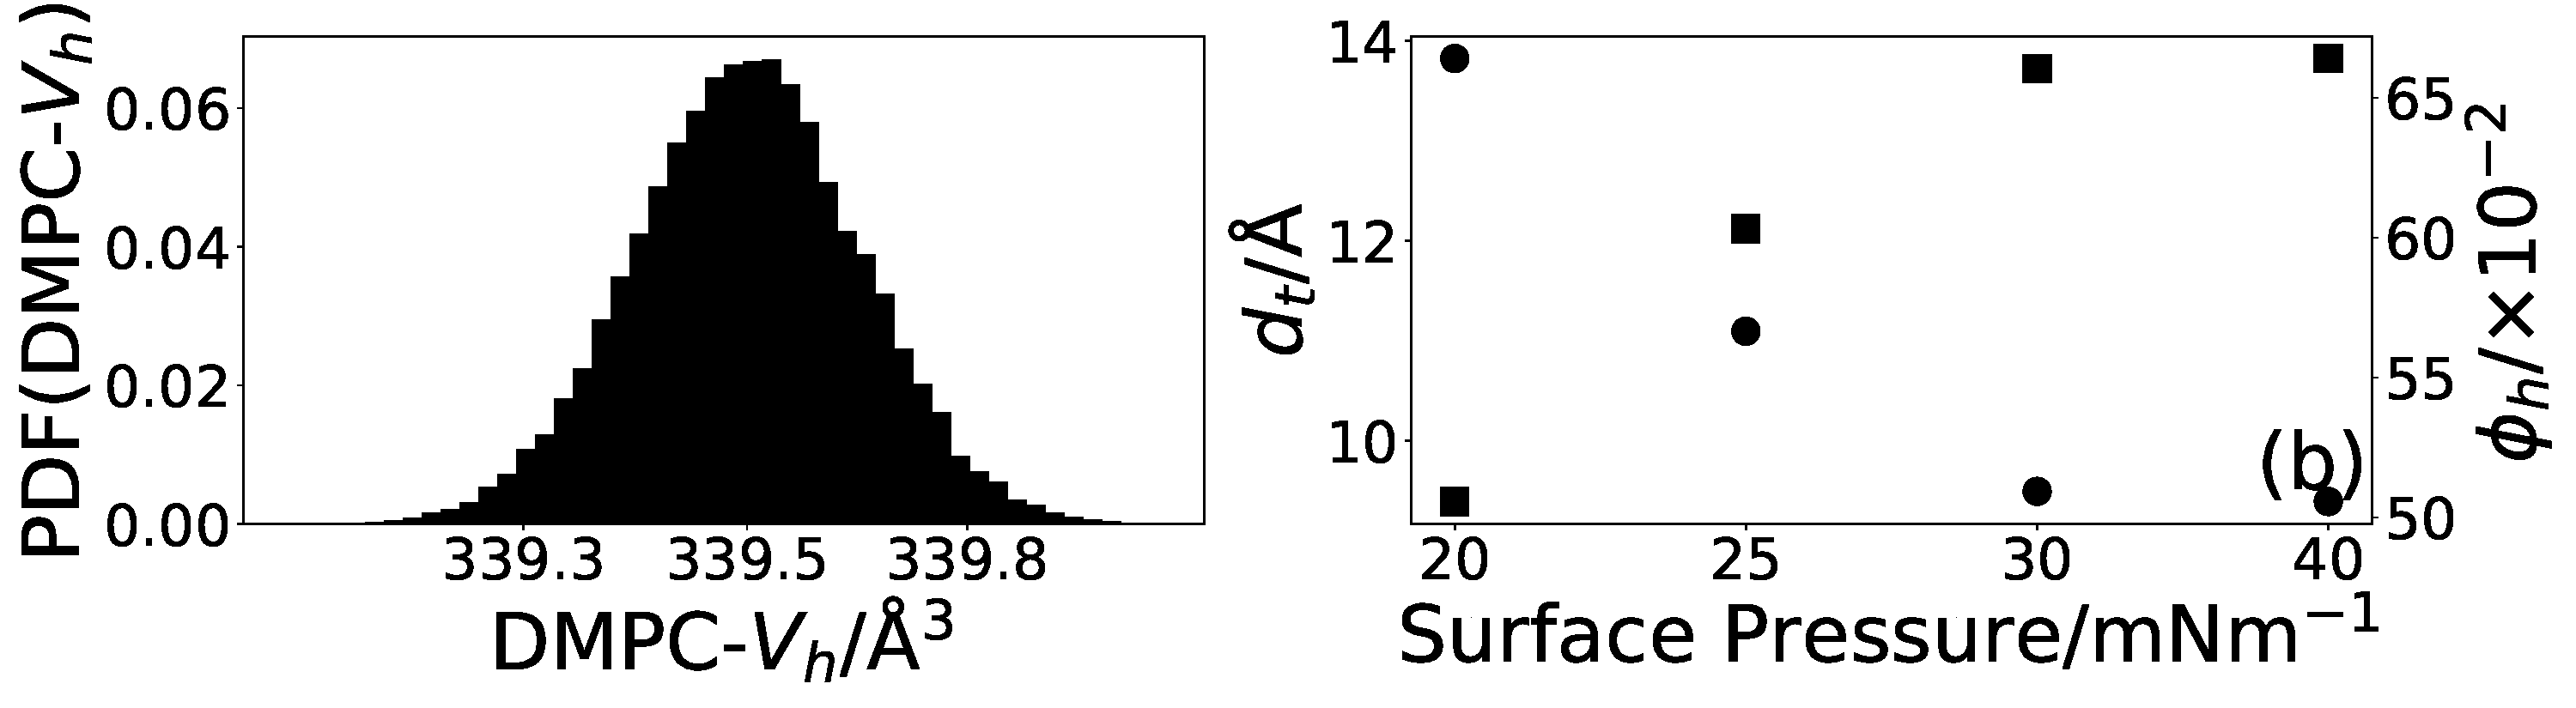
\includegraphics[width=0.45\textwidth]{figures/dmpc_vh_dt_phi}
	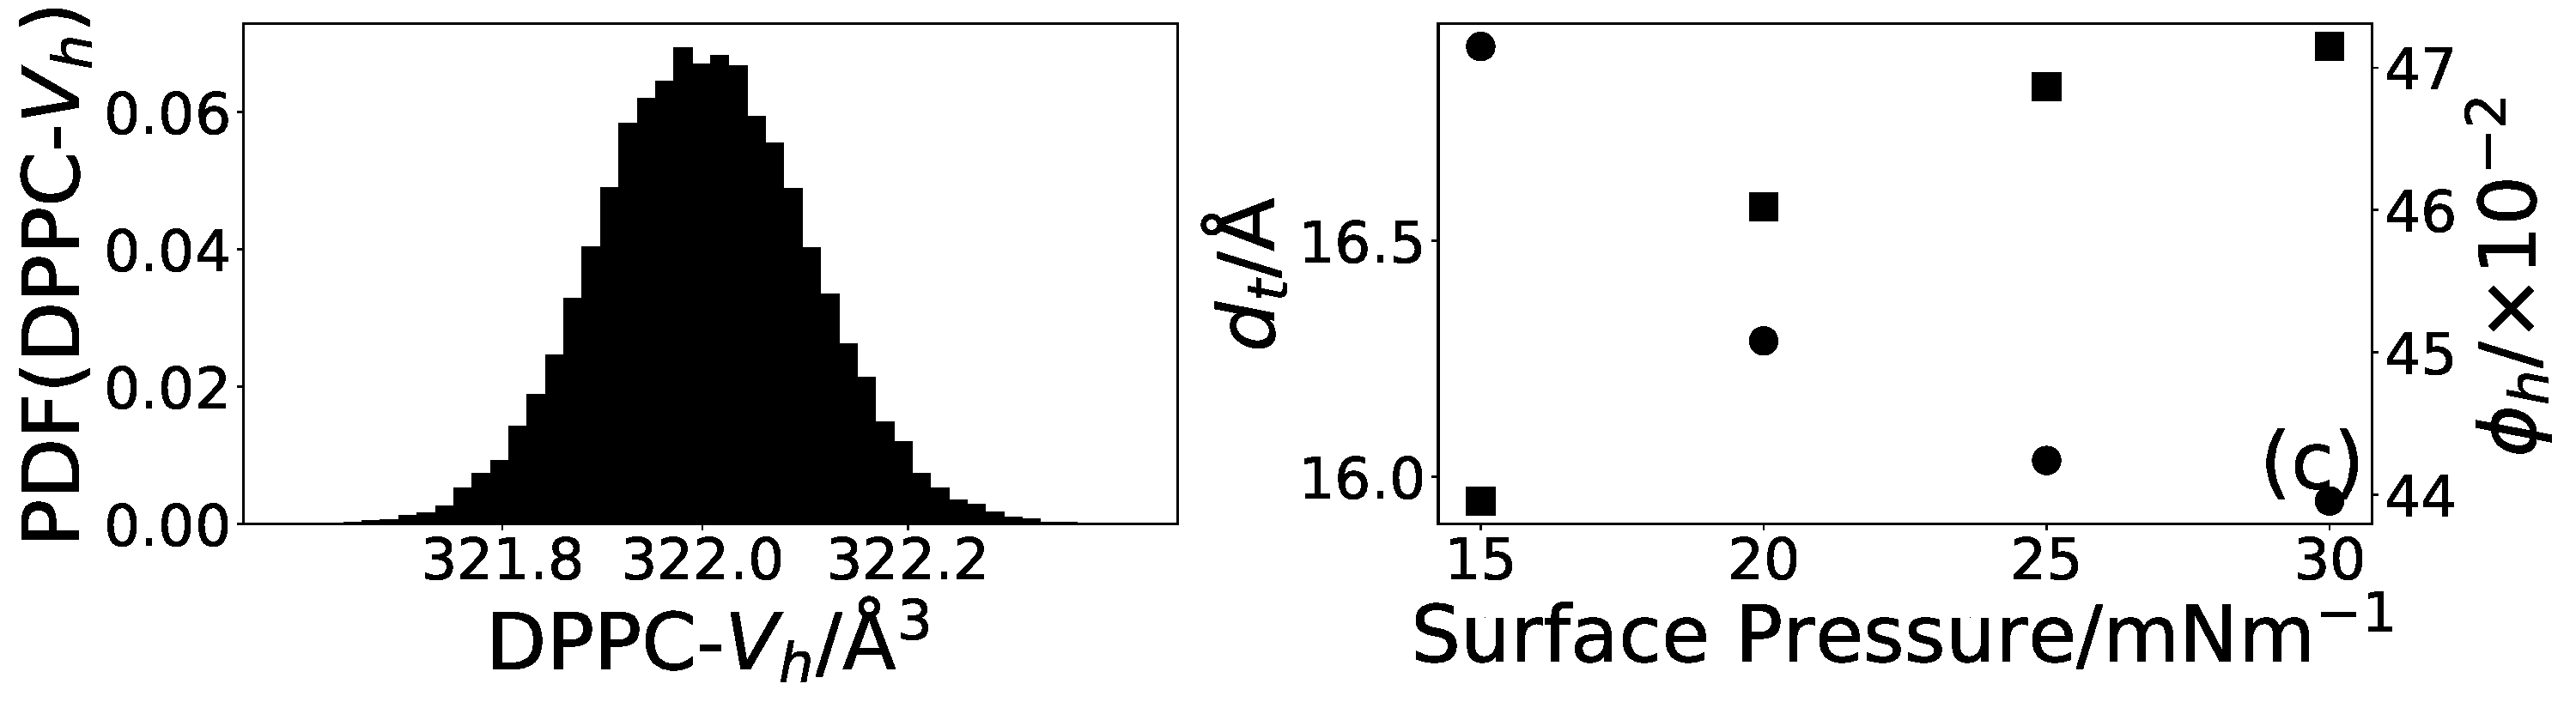
\includegraphics[width=0.45\textwidth]{figures/dppc_vh_dt_phi}
	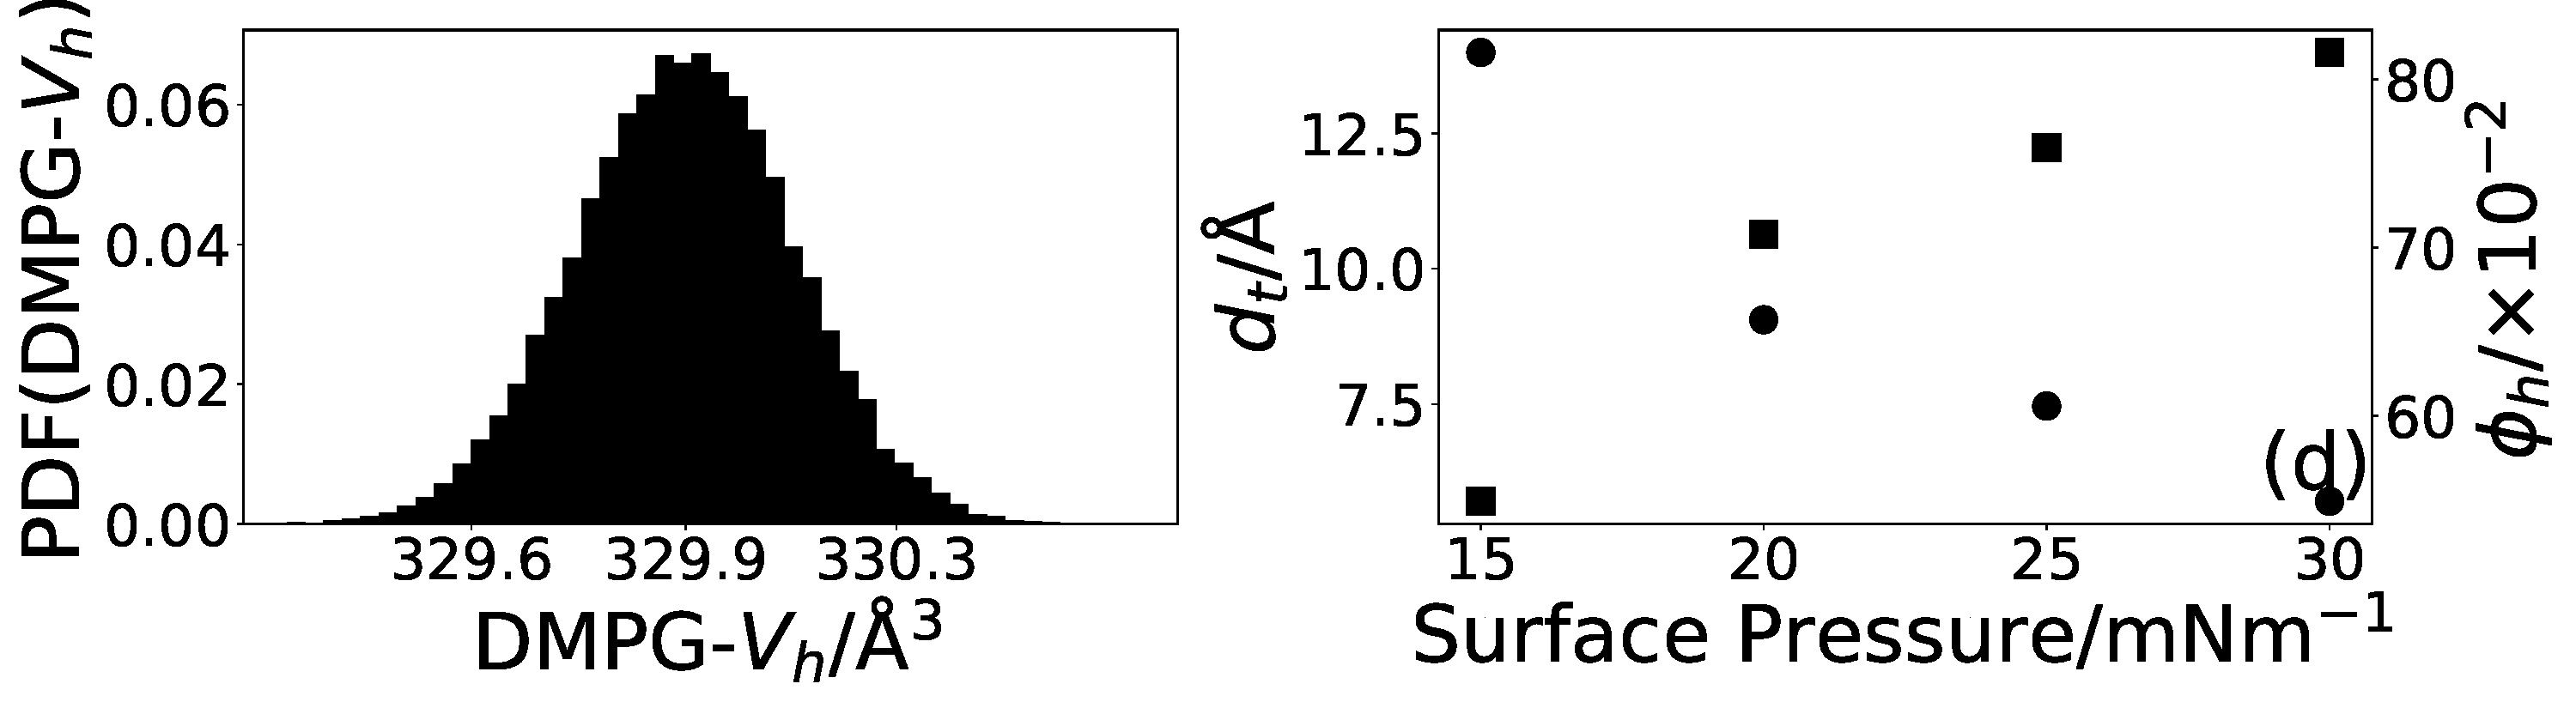
\includegraphics[width=0.45\textwidth]{figures/dmpg_vh_dt_phi}
	\caption{\small The PDFs of the head volume (left) and variation of
  $d_t$ (squares) and $\phi_h$ (circles) with surface pressure for each of
  the four lipids; (a) DLPC, (b) DMPC, (c) DPPC, (d) DMPG. The values of
  $d_t$ were found from the appropriate values of $\theta_t$ using
  Eqn. \ref{equ:tl}.}
	\label{fig:lipresults}
\end{figure}
%

Figure \ref{fig:lipresults} also shows that for all four lipids there is a
decrease in head solvation, $\phi_h$, with surface pressure.
This is because an increase in the surface pressure means a reduction in the
free volume available between the lipid heads, which in turn forces solvent
molecules out of the layer, an effect that has also been observed on
water\cite{Bayerl1990}.

Our fits suggest lower lipid tail volumes than previous measurements using
other techniques (compare Tables \ref{tab:water} and \ref{tab:liptab}).
It is unlikely that this is a result of the DES subphase since the tails do
not directly interact with the solvent.
However this may be related to the compaction of the monolayer at elevated
surface pressures.
The optimal value of the tail volume for DPPC in the LC
phase\cite{Campbell2018} was found to be \SI{772}{\cubic\angstrom} at
\SI{35}{\milli\newton\per\meter}, which agrees well with the value of
\input{../output/dppc/vt.txt}\si{\cubic\angstrom} found in this work.
Similarly the tail volume for DMPS in the LE phase\cite{Campbell2018},
\SI{714}{\cubic\angstrom} at \SI{10}{\milli\newton\per\meter}, broadly
agrees with the values for
DMPC (\input{../output/dmpc/vt.txt}\si{\cubic\angstrom}) and DMPG
(\input{../output/dmpg/vt.txt}\si{\cubic\angstrom}) in this work.
The literature value\cite{Pan2012} quoted for DMPG (at a lower temperature) is
also similar to our result (but slightly smaller).
We find that the reduction is \SIrange{8}{12}{\percent} for DPPC, DMPC and
DLPC when compared with literature sources at \SIrange{24}{30}{\celsius}, in
good agreement with the maximum compression percentage of \SI{15}{\percent}
noted by Small \emph{et al.}\cite{Small1984}.
In general our results are at least self-consistent while comparisons to the
literature are favourable.

Figure \ref{fig:lipresults} shows the PDFs for the head volume for each of
the four lipids.
The three lipids with the PC head are consistent with values of around
\SI{330}{\cubic\angstrom}, regardless of hydrocarbon tail.
This agrees well with the values found for the same head in water
(Table \ref{tab:water}).
Interestingly, the volume for the PG head is similar to that for the PC head
with a value of \input{../output/dmpg/vh.txt}\si{\cubic\angstrom}, which is
significantly larger than values quoted in the literature for
DMPG\cite{Pan2012} (\SI{291}{\cubic\angstrom}) or POPG\cite{Kucerka2012}
(\SI{289}{\cubic\angstrom}).
This suggests that there may be some effect arising from the solvation in DES.

The major difference between the two heads is the fact PG head is negatively
charged whereas the PC head is zwitterionic (Figure \ref{fig:heads}).
It has been shown previously that the PC head is folded in
water\cite{Gilliams2016}, while the presence of strong electrostatic
interactions in DES is known to effect the structure of surfactants
micelles\cite{Sanchez-Fernandez2018}.
If we infer a similar folded structure for the PG head driven by a weaker
interaction between the alcohol and phosphate groups, then we may explain
the observed increase in volume to be due to unfolding of the PG head
because we expect that the DES provides a greater charge screening effect
than water.
If so then we would also expect an increase in the thickness of the head
layer in DES. This does seem to be the case: The PG head layer thickness was
found to be \SI[separate-uncertainty=true]{10.3\pm0.4}{\angstrom} at
\SI{22}{\milli\newton\per\meter} \cite{Clifton2012} and
\SI[separate-uncertainty=true]{9.7\pm1.0}{\angstrom} at
\SI{15}{\milli\newton\per\meter} \cite{Ciumac2017} from NR measurements at
the air-water interface.
For the PC head the stronger folding interaction, due to the formal charge
on the ammonium group, means that no unfolding effect is observed.

The volumes determined for the head and tails, and the thickness of the head
layers, for DMPC and DPPC were used to constrain the fitting of corresponding
NR data (Figure \ref{fig:neutron}). This leaves only two variables,
$\theta_t$ and $\sigma$ to fit this data.
The agreement is good and a confirmation that the volumes derived from XRR
are consistent with the NR data.
Furthermore, the observed trends with surface pressure are also consistent
which adds some confidence in our conclusions.
%
\begin{figure}
	\centering
  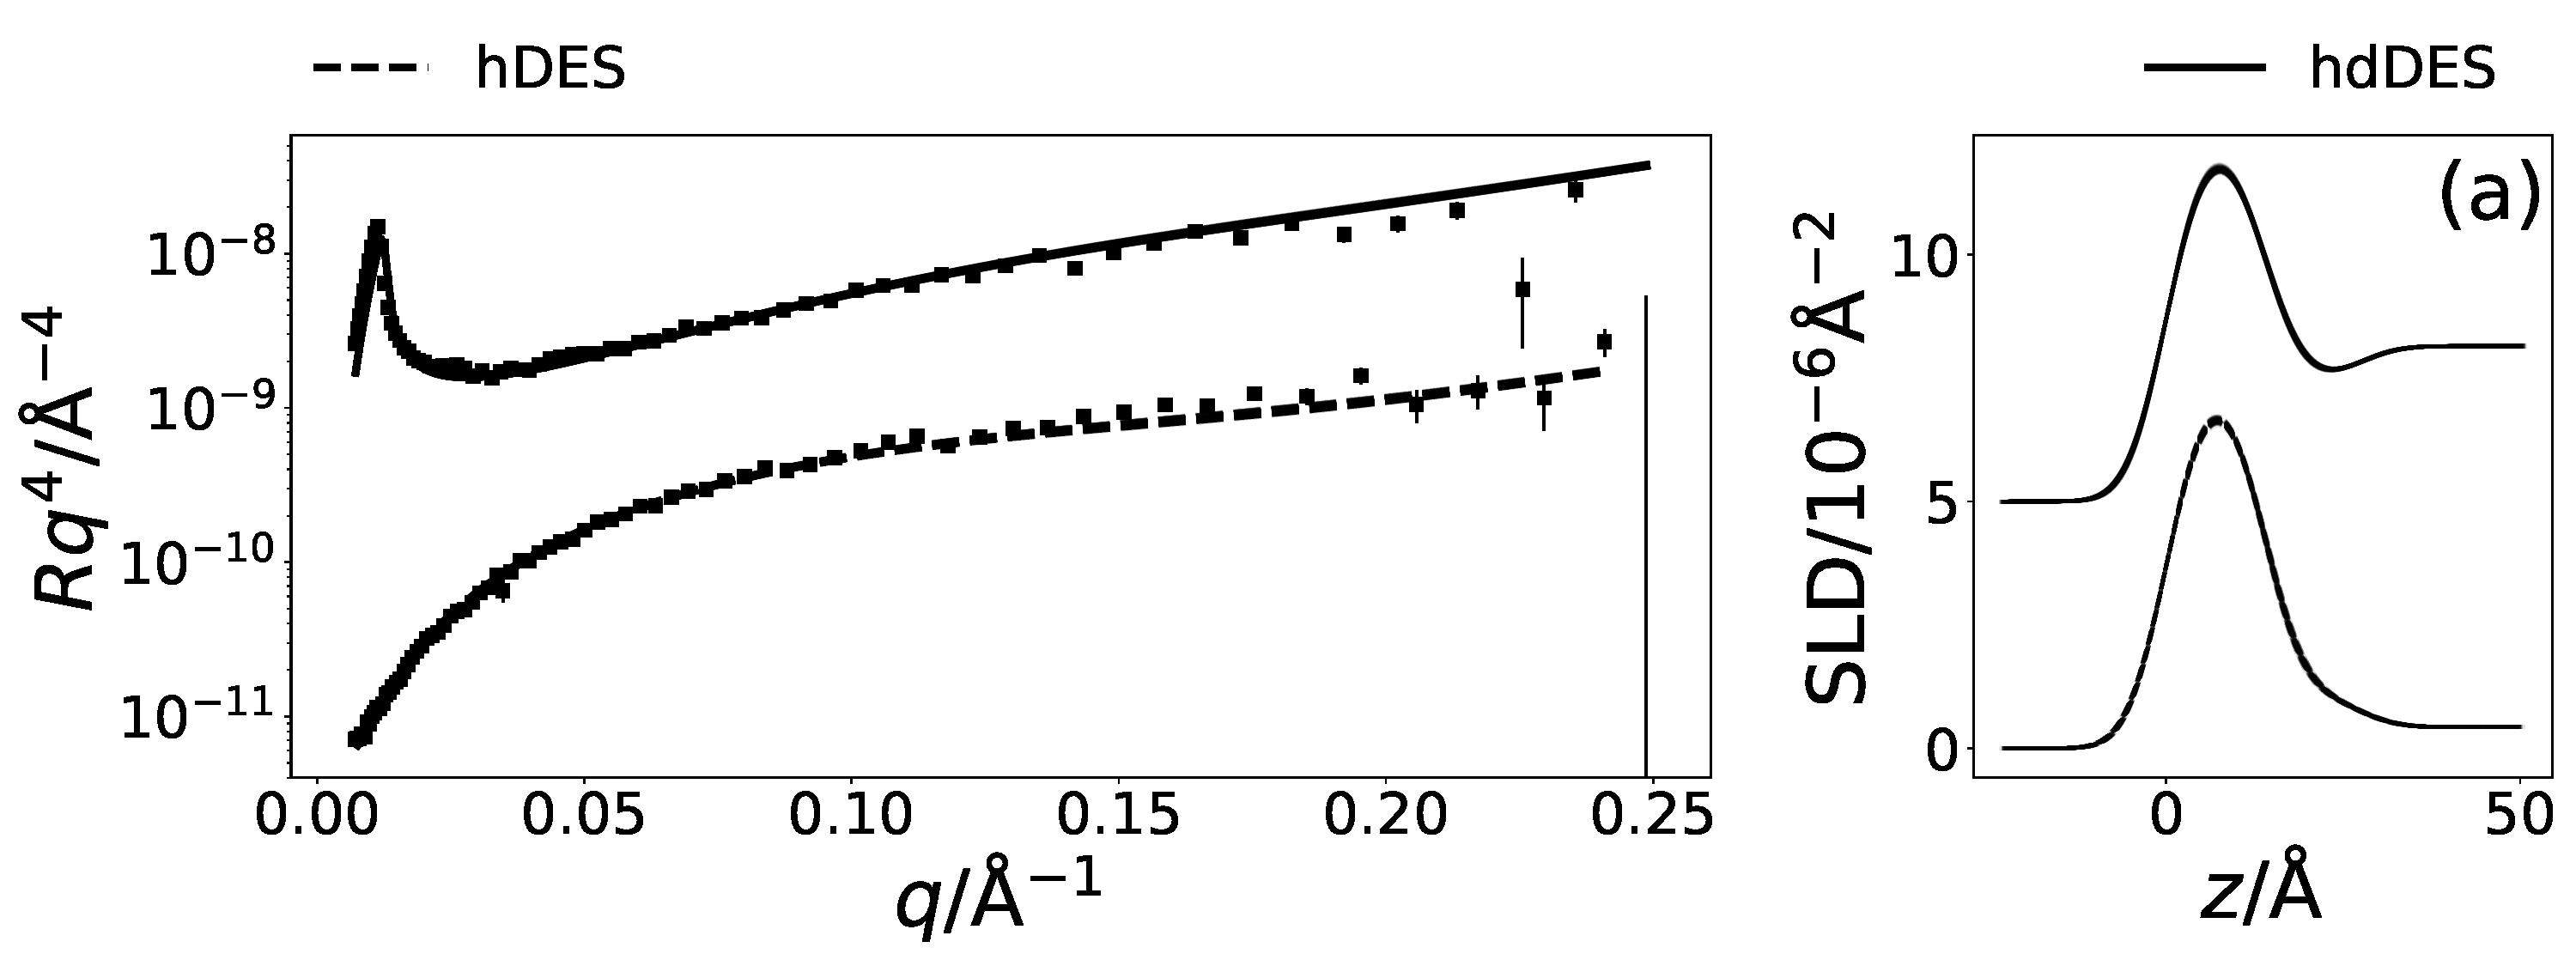
\includegraphics[width=0.45\textwidth]{figures/dmpc_20n_ref_sld}
	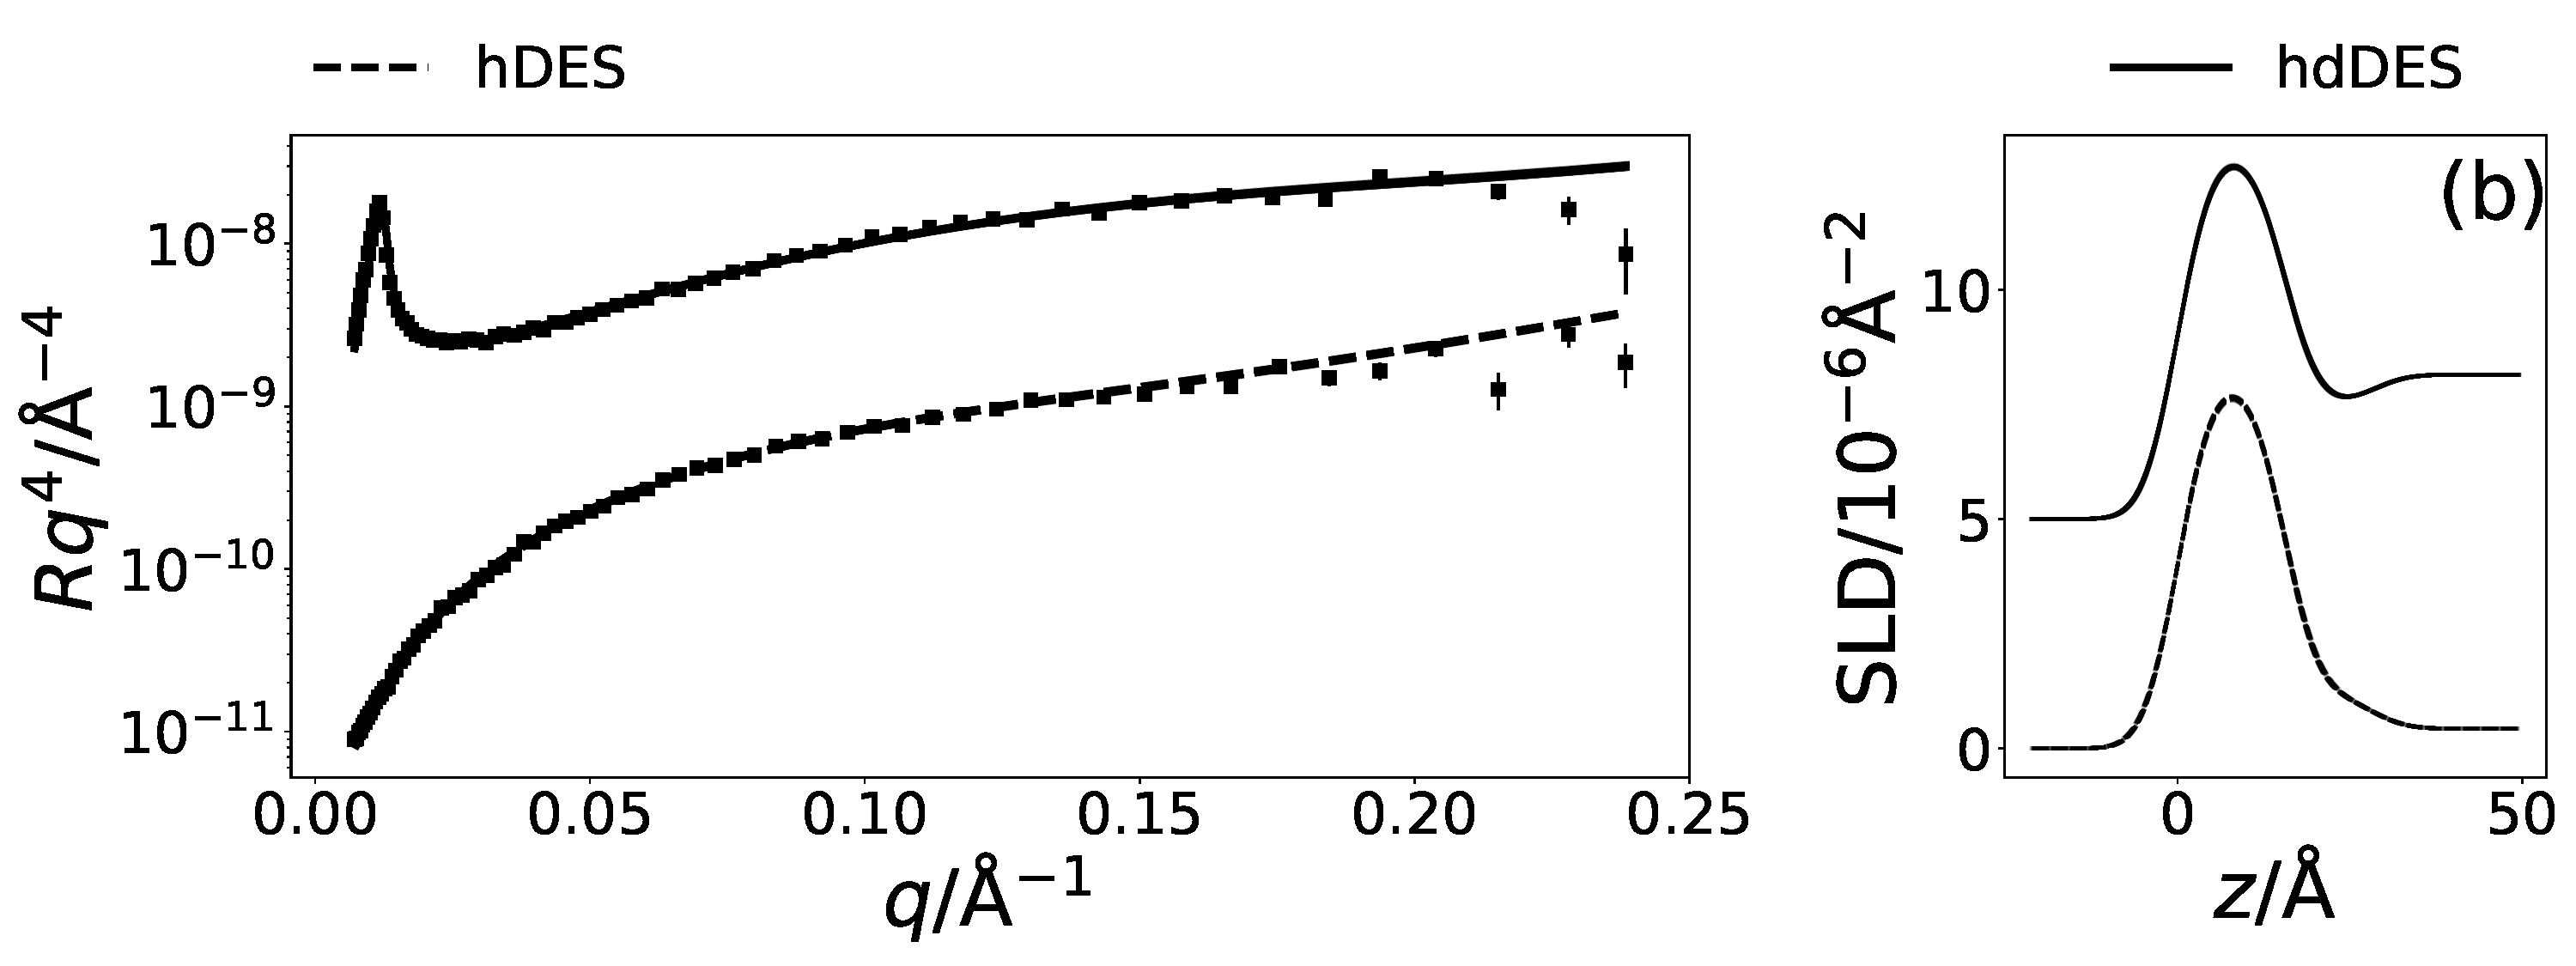
\includegraphics[width=0.45\textwidth]{figures/dppc_20n_ref_sld}
	\caption{\small The NR and SLD profiles at a surface pressure of
  20 mNm$^{-1}$ for two contrasts (see legend above each plot); (a) DMPC,
  (b) DPPC. The NR profiles have been offset in the $y$-axis by an order of
  magnitude and SLD profiles offset in the $y$-axis by
  \SI{5e-6}{\per\square\angstrom}, for clarity.}
	\label{fig:neutron}
\end{figure}
%
%
\begin{table}
  \caption{\label{tab:neutron} The best-fit values, and associated 95 \%
  confidence intervals for the varying parameters in the co-refined NR models.
  The values of $d_t$ were found from the appropriate values of $\theta_t$
  using Eqn. \ref{equ:tl}, and the values of $\phi_h$ were found using Eqn.
  \ref{equ:phih}.}
  \begin{ruledtabular}
	\begin{tabular}{ccccc}
    Lipid & \multicolumn{2}{c}{d$_{54}$-DMPC} & \multicolumn{2}{c}{d$_{62}$-DPPC} \\
    SP/mNm$^{-1}$ & 20 & 25 & 15 & 20 \\
    \hline
    $\theta_t$/$^\circ$ & \input{../output/dmpc/angle20_neutron.txt} &
    \input{../output/dmpc/angle25_neutron.txt} &
    \input{../output/dppc/angle15_neutron.txt} &
    \input{../output/dppc/angle20_neutron.txt} \\
    $\sigma_{t,h,s}$/\AA & \input{../output/dmpc/rough20_neutron.txt} &
    \input{../output/dmpc/rough25_neutron.txt} &
    \input{../output/dppc/rough15_neutron.txt} &
    \input{../output/dppc/rough20_neutron.txt} \\
    \hline
    $\phi_h$/$\times10^{-2}$ & \input{../output/dmpc/solh20_neutron.txt} &
    \input{../output/dmpc/solh25_neutron.txt} &
    \input{../output/dppc/solh15_neutron.txt} &
    \input{../output/dppc/solh20_neutron.txt} \\
    $d_t$/\AA & \input{../output/dmpc/tail20_neutron.txt} &
    \input{../output/dmpc/tail25_neutron.txt} &
    \input{../output/dppc/tail15_neutron.txt} &
    \input{../output/dppc/tail20_neutron.txt} \\
	\end{tabular}
  \end{ruledtabular}
\end{table}
%

For the first time, stable phosphocholine and phosphatidylglycerol lipid
monolayers have been observed and characterised on a non-aqueous liquid
surface.
Until the emergence of ionic liquids and DES, only a limited number of
molecular solvents exhibited the ability to promote self-assembly and, to
the best of our knowledge, only water among those had demonstrated the
formation of functional phospholipid monolayers at the air-liquid interface.

A physically and chemically constrained modelling approach and Bayesian
analysis method was used to rationalise these measurements showing that the
structures are remarkably similar at the air-DES interface to those
previously observed at the air-water interface.
This has the important implication that DES therefore offer the possibility
of performing studies of model membranes in the absence of water.
Such applications may include fundamental investigations of phospholipid
monolayers in extreme environments (total or partial absence of water,
cryogenic temperatures), protein membrane interactions and development of
new technologies for drug delivery.
However, the fact remains that the PG lipid did show a significant
difference; having a larger head volume than observed for the same system
in water.
This shows that the transfer of lipids to a DES is not just a simple
substitution of the subphase. In this specific case we have proposed an
explanation based on unfolding of the PG head that is enabled by
electrostatic screening of the head charges by the charged solvent.

The ability to determine the head volume was facilitated by access to easy to
use, and open-source software that allowed for the straightforward use a
custom, chemically-consistent model within the analysis of the XRR and NR
measurements.
Furthermore, this work presents the first, to our knowledge, use of
chemically-consistent parameterisation to co-refine XRR measurements at
different surface concentrations.

\begin{acknowledgments}
The authors thank Andrew Nelson for their help with the refnx software.
A.R.M. is grateful to the University of Bath and Diamond Light Source for
co-funding a studentship (Studentship Number STU0149).
Thanks also to the European Spallation Source and the University of Bath
Alumni Fund for supporting A.S.-F.
We also thank Diamond Light Source (Experiment number SI10546-1) and
Institut Laue-Langevin (DOI:
\href{http://doi.org/10.5291/ILL-DATA.9-13-612}{10.5291/ILL-DATA.9-13-612})
for the awarded beamtime.
\end{acknowledgments}

\bibliography{bibi}% Produces the bibliography via BibTeX.

\end{document}
